\newpage

\section{Hinderniserkennung}

Wie bereits im \acrshort{pren1} klar wurde, ist das Problem der Hinderniserkennung zu komplex, um mit simpler Bildverarbeitung gelöst werden zu können. 
Das Erkennen von Objekten auf einem Bild, wurde bereits durch \acrfull{cnn} gelöst.

\subsection{Objektdetektierung mit \acrshort{cnn}}

Die Objektdetektierung ist eines von vier Grundproblemen des {\it Computer Vision} Forschungsbereiches.
Dazu zählen die Bildklassifizierung, Objektdetektierung, Semantische Segmentation und Instance Segmentation.

\image{img/CNN/computer-vision-research-fields}
{
Der Forschungsbereich der {\it Computer Vision} \cite{wu2019recent} besteht aus Bildklassifizierung, 
Objektdetektierung, Semantische Segmentation und Instance Segmentation.
}

\newpage

Bei der Objektdetektierung werden einzelne Objekte einer bestimmten Klasse mit {\it Bounding Boxes}
eingezeichnet. Die Genauigkeit solcher \acrshort{cnn} kann für ein spezialisiertes Gebiet die
eines Menschen übertreffen \cite{BUETTIDINH2019e00321}.

\subsection{Algorythmen zur Objektdetektierung}

Es gibt verschiedene Algorithmen zur Detektierung von Objekten in einem Bild. 
Dabei ist vor allem die Abwägung zwischen Genauigkeit und Geschwindigkeit entscheidend.
Aus diesem Grund wird die Objektdetektierung auch in zwei Gruppen unterteilt, nämlich 
(i) single-stage detection wie \acrshort{yolo} \cite{redmon2016look} oder \acrshort{ssd} \cite{Liu_2016} und (ii) two-stage detection wie \acrfull{r-cnn} \cite{girshick2015fast}.

Ein two-stage detector besteht aus einem ersten Feature Proposal Schritt, gefolgt von einer Klassifizierung der vorgeschlagenen Features des ersten Schrittes. Ein sigle-stage Detector klassifiziert die Regionen eines Bildes direkt in einem Durchlauf. 

Während single-stage Detektoren generell eine schnelleres Inference bieten, sind two-stage Detektoren genauer \cite{soviany2018optimizing}.
Aus diesem Grund werden häufig für Echtzeitanwendungen Objektdetektierung, wie das Erkennen von Objekten in einem Videostream, single-stage
Detektoren verwendet.

\subsection{\acrfull{r-cnn}}

Aufgrund der erhöhten Genauigkeit von two-stage Detektoren, wird in dieser Arbeit vor allem \acrshort{r-cnn} behandelt.

Bei einem \acrshort{r-cnn} \cite{girshick2014rich} werden als Erstes interessante Regionen von einem \acrshort{cnn} für die 
spätere Segmantische Kategorisierung vorgeschlagen. Laut dem Paper von \acrshort{r-cnn}, wird eine um 30\% erhöhte Genauigkeit 
gegenüber vorherigen Objekterkennungsalgorythmen auf dem VOC 2012 Datenset erreicht. Damit wird eine \acrfull{map} von 53.3\%
auf dem VOC 2012 Datenset erreicht.

Bei einem \acrshort{r-cnn} 

\image{img/CNN/r-cnn}
{
  Der \acrfull{r-cnn} \cite{girshick2014rich} Objektdetektierungs Algorythmus bei welchem zuerst Regionen 
  vorgeschlagen werden, auf denen danach mit einem Backbone Segmantische Kategorisierung durchgeführt wird und
  das Objekt einer Klasse zugeteilt wird.
}

\subsection{Erkennung von Ziegelsteinen und Treppenstufen}

\subsubsection{Vereinfachtes \acrshort{r-cnn}}

Ein erster simpler Versuch die Hindernisse (Ziegelsteine) zu erkennen war, mittels Feature Engineering\footnote{
In diesem Fall wurde Canny Edge detection \cite{canny-edge-detection} angewendet}, die Treppenstufen zu
erkennen. Ein Sliding Window auf der Treppenstufe dient dabei als Feature Proposal.
Die Kategorisierung wurde mit einem einfachen \acrshort{cnn} basierend auf den Sliding Window features 
realisiert.

\image{img/CNN/sliding-window-stair}
{
Ansatz eines vereinfachten \acrshort{r-cnn} mit Stufenerkennungs Feature engineering.
}

Die Resultate konnten weder die erwartete Performanz noch Genauigkeit zufriedenstellen.
Das Paper dazu kann auf GitHub \footnote{
https://github.com/randombenj/hslu-pren/blob/a987e1c53f3b44a86b42ca3030afb1f12880d94c/pren1/research/yes-no-classification-sliding-window.ipynb} gefunden werden.


\subsubsection{Detectron2}

Detectron2 \cite{wu2019detectron2} ist ein State of the Art Framework für Objektdetektierung, Semantische- und Instance Segmentierung.
Es werden verschiedene \acrshort{r-cnn} Models zur verfügung gestellt. \footnote{
\url{https://github.com/facebookresearch/detectron2/blob/master/MODEL_ZOO.md#coco-object-detection-baselines}
}
Zudem bietet Detectron2 eine sehr einfache Möglichkeit mittels Transfer Learning \footnote{
\url{https://colab.research.google.com/drive/16jcaJoc6bCFAQ96jDe2HwtXj7BMD_-m5#scrollTo=b2bjrfb2LDeo}
}
einen eigenen Datensatz, bestehend auf dem vortrainierten Gewichten der Features zu trainieren.
Somit ist es möglich, mit wenigen hundert Bildern neue Objekte zu erkennen.

\subsubsection{Performance Testing}

Um zu sehen ob ein Raspberry Pi solch komplexes \acrshort{cnn} überhaupt berechnen kann, oder ob ein
Leistungsfähigeres Compute Board gekauft werden muss, werden Performance Tests durchgeführt.
Das Setup für die Performancetests kann auf GitHub \footnote{\url{https://github.com/randombenj/detectron2onnx-inference/blob/master/detectron2-onnx.ipynb}} gefunden werden.

Für die Performancetests werden drei Controller angeschaut, die Controller konnten ausgeliehen werden.

\begin{itemize}
    \item Raspberry Pi
    \item Jetson Nano (4GB)
    \item Jetson TX1
\end{itemize}

\image{img/CNN/boards}{
Das Jetson TX1 (unten), Jetson Nano (oben mitte) und das Raspberry Pi (oben rechts und links)
}

Die Performancetests wurden mit dem oben genannten Notebook durchgeführt, zusätzlich werden die Zeiten für die
Inference gemessen. Die gemessenen Resultate sind:

\begin{itemize}
    \item {\bf Raspberry Pi}  ~500s
    \item {\bf Jetson Nano (4GB)} ~10s
    \item {\bf Jetson TX1} ~2s
\end{itemize}

Zwar können mit Optimierung (durch das einsetzen von ONNX)\footnote{https://onnx.ai/} beim Raspberry Pi eine Inference Zeit von ~20s erreicht werden, 
dann sind aber alle vier CPU Kerne zu 100\% für die gesamte Zeit ausgelastet.

Da die Nvidia Boards jeweils über eine Maxwell GPU verfügen und diese auch mit CUDA \footnote{https://developer.nvidia.com/cuda-zone}
für Machine Learning verwendet werden kann, wurde entschieden, das Jetson Nano anstatt das ursprünglich geplante
Raspberry Pi zu besorgen. Das Jetson Nano verfügt über die gleichen Kamera und GPIO Anschlüsse, und 
ist somit Kompatibel mit der geplanten Elektronik.

\subsection{Trainieren des \acrshort{cnn}}

Bei den detectron2 \acrshort{cnn} Modellen kann ein bereits vortrainiertes Neuronales Netz
verwendet werden. Dieses kann anschliessend mit wenigen hundert Bildern via Transfer Learning \footnote{https://en.wikipedia.org/wiki/Transfer\_learning}
auf ein eigenes Datenset angepasst werden.

Den Vorgang kann man sich so vorstellen, dass das Modell verschiedene, häufig vorkommende Formen wie Kreise, Vierecke, ...
bereits kennt und man durch das Datenset dem Modell beibringt was eine Treppenstufe oder ein Ziegelstein ist.

\subsubsection{Sammeln von Trainingsdaten}

Die Trainingsdaten werden mithilfe eines Kartonprototypen und einer selbsprogrammierten App gesammelt.
Im Kartonprototypen wurde die Kamera auf der gleichen Höhe und im gleichen Winkel eingebaut
wie im Prototypen.
Mithilfe der App auf dem Gerät, können über das Smartphone einfach Bilder aufgenommen werden.

Die Bilder wurden in einer Auflösung von 720x960 Pixel aufgenommen. Ziel war es, etwa 300 Bilder zu sammeln um für das \acrshort{cnn} zu annotieren.

\image{img/CNN/pren-image-capture}{
Aufnahme der Trainingsdaten für die Hinderniserkennung
}

\subsubsection{Annotieren der Trainingsdaten}

Die Trainingsdaten wurden nach dem Aufnehmen mithilfe von COCO Annotator \footnote{https://github.com/jsbroks/coco-annotator} annotiert.
Dabei wurden zwei Klassen verwendet: {\it Brick} und {\it Stair}.

\image{img/CNN/coco-stair}{
Annotieren der Trainingsdaten im COCO Datenformat \footnote{\url{https://cocodataset.org/#format-data}}.
}

\subsubsection{Trainieren des \acrshort{cnn}}

Als vorlage für das Trainieren wurde das offizielle Notebook von detectron2 verwendet. \cite{detectron2-colab}

Um das \acrshort{cnn} zu trainieren und auch die Performance zu evaluieren, werden die annotierten Trainingsdaten
in Train- (70\%), Test- (20\%) und Validationsset (10\%) unterteilt.

Die Trainingsdaten dienen dazu, dass Model zu trainieren. Mit den Testdaten werden die Hyperparameter\footnote{\url{https://en.wikipedia.org/wiki/Hyperparameter_(machine_learning)}} verfeinert und
mit dem Validationsset wird am Schluss die Performance des \acrshort{cnn} gemessen.

Die verschiedenen Datensätze werden dem detectron2-trainer bekanntgegeben:

\begin{minted}{python}
from detectron2.data.datasets import register_coco_instances

DatasetCatalog.clear()

register_coco_instances("stair_train", {}, "stair-train.coco.json", "stair/")
register_coco_instances("stair_test", {}, "stair-test.coco.json", "stair/test/")
register_coco_instances("stair_validation", {}, "stair-validation.coco.json", "stair/validation/")
\end{minted}

Das Model wird wie folgt vorkonfiguriert:

\begin{minted}{python}
model_config = "COCO-Detection/faster_rcnn_R_50_FPN_3x.yaml"

cfg = get_cfg()

# add project-specific config (e.g., TensorMask) here if you're not running a model in detectron2's core library
cfg.merge_from_file(model_zoo.get_config_file(model_config))
cfg.MODEL.ROI_HEADS.SCORE_THRESH_TEST = 0.5  # set threshold for this model

# Find a model from detectron2's model zoo. You can use the https://dl.fbaipublicfiles... url as well
cfg.MODEL.WEIGHTS = model_zoo.get_checkpoint_url(model_config)

cfg.INPUT.MAX_SIZE_TRAIN = 480
cfg.INPUT.MAX_SIZE_TEST = 480

cfg.OUTPUT_DIR = 'outputs/480_no_aug_4_im_batch'
cfg.DATASETS.TRAIN = ("stair_train",)
cfg.DATASETS.TEST = ("stair_test",)

cfg.TEST.EVAL_PERIOD = 25  # evaluate test set (validation) every X periods.
cfg.VIS_PERIOD = 25  # visualize a sample image every X periods.

# limit the amount of memory the GPU can allocate
# fixes, RuntimeError: CUDA out of memory.
cfg.SOLVER.IMS_PER_BATCH = 8
#cfg.SOLVER.BASE_LR = 0.02
cfg.SOLVER.MAX_ITER = 1000

cfg.MODEL.ROI_HEADS.NUM_CLASSES = 2  #  classes (stair, brick)
\end{minted}

Nun kann das Model trainiert werden:

\begin{minted}{python}
trainer = DefaultTrainer(cfg)
trainer.resume_or_load(resume=False)
trainer.train()
\end{minted}


\begin{figure}[H]
  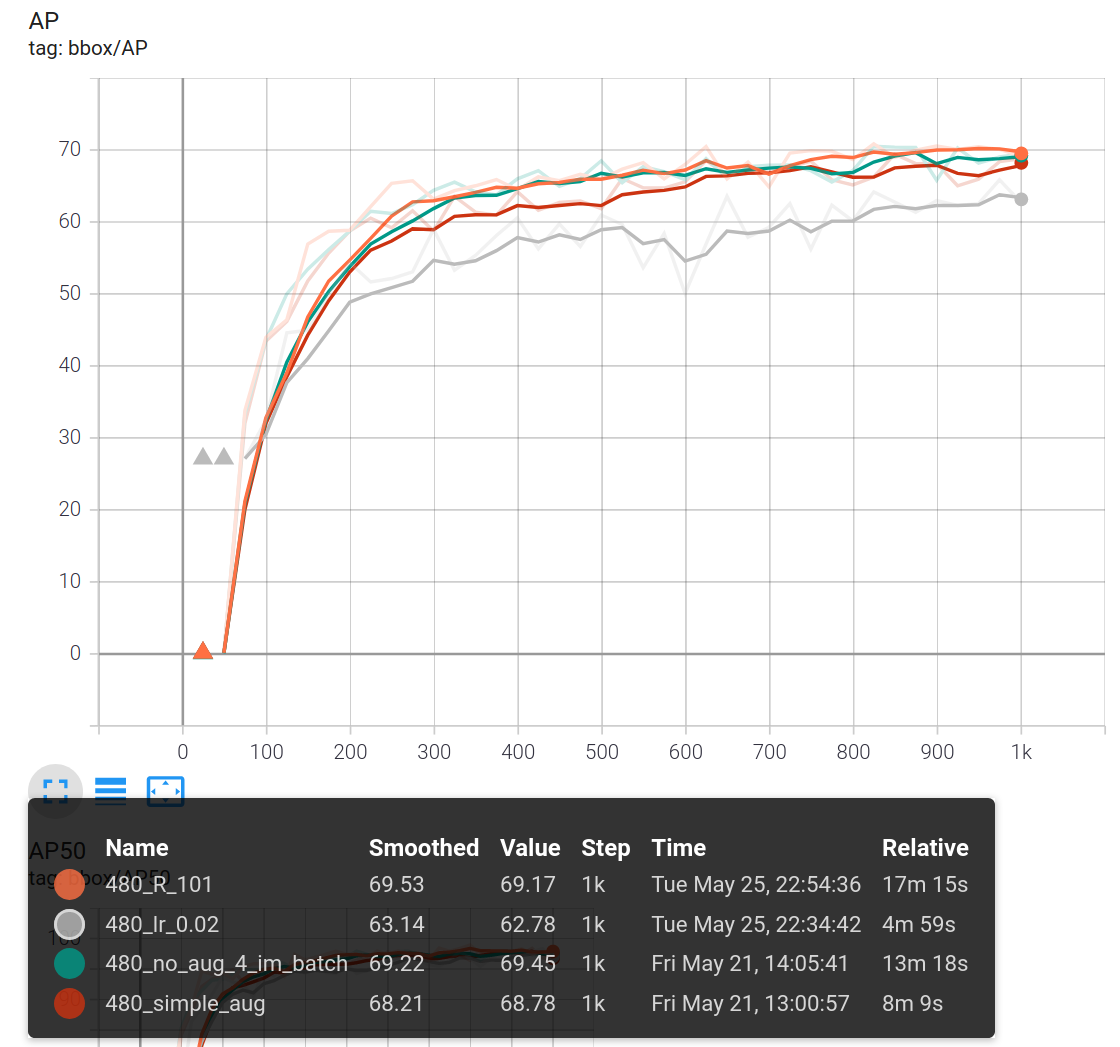
\includegraphics[width=0.95\textwidth]{img/CNN/model-accuracy.png}
  \caption{Die accuracy zeigt die Performance des Models während der Trainingsphase an.}
  \label{fig:model-performance}
\end{figure}

Wie in \ref{model-performanc} gezeigt, wurden verschiedene Konfigurationen ausprobiert 
(sogenanntes Hyperparameter tuning \footnote{\url{https://en.wikipedia.org/wiki/Hyperparameter_(machine_learning)}}).

Am Schluss wurde das Model mit der besten Performance ausgewählt, welches nicht overfitted war.
Overfitting hat sich durch 'False positives gezeigt', beispielsweise Ziegelsteine und Treppenstufen erkennen die gar nicht im
Bild sind.

Data-Augmentation \cite{perez2017effectiveness} hatte keinen grossen Einfluss auf die Performance des Models
oder hat diese sogar noch schlechter gemacht.

\subsection{Model Performance}

Um die Perofmance des Models zu messen, werden die 'Truely unseen Validationdata' verwendet:

\begin{minted}{python}
from detectron2.data import DatasetCatalog, MetadataCatalog, build_detection_test_loader
from detectron2.evaluation import COCOEvaluator, inference_on_dataset

evaluator = COCOEvaluator("stair_validation", cfg, False, output_dir="./output/")
val_loader = build_detection_test_loader(cfg, "stair_validation")

inference_on_dataset(trainer.model, val_loader, evaluator)
\end{minted}

Dabei werden die Validationsdaten durch das Model Annotiert und danach mit den 'Ground Truth' Daten 
(also den Manuellen Annotations) verglichen. Dies ergibt danach einen Performance Report.

\begin{minted}{text}
|   AP   |  AP50  |  AP75  |  APs   |  APm   |  APl   |
|:------:|:------:|:------:|:------:|:------:|:------:|
| 70.880 | 99.019 | 87.718 | 70.000 | 62.991 | 77.799 |
\end{minted}

\begin{minted}{text}
| category   | AP     | category   | AP     |
|:-----------|:-------|:-----------|:-------|
| stair      | 74.730 | brick      | 67.031 |
\end{minted}

Anhand der Validationsdaten kann die Performance des Models ersichtlich gemacht werden.

\image{img/CNN/pren-inference-example}{
Anhand der Validationsdaten, welche das \acrshort{cnn} vorher noch nie gesehen hat, 
kann die zu erwartende Performance abgeschätzt werden. 
}

\section{Pfadberechnung}

\begin{figure}[H]
  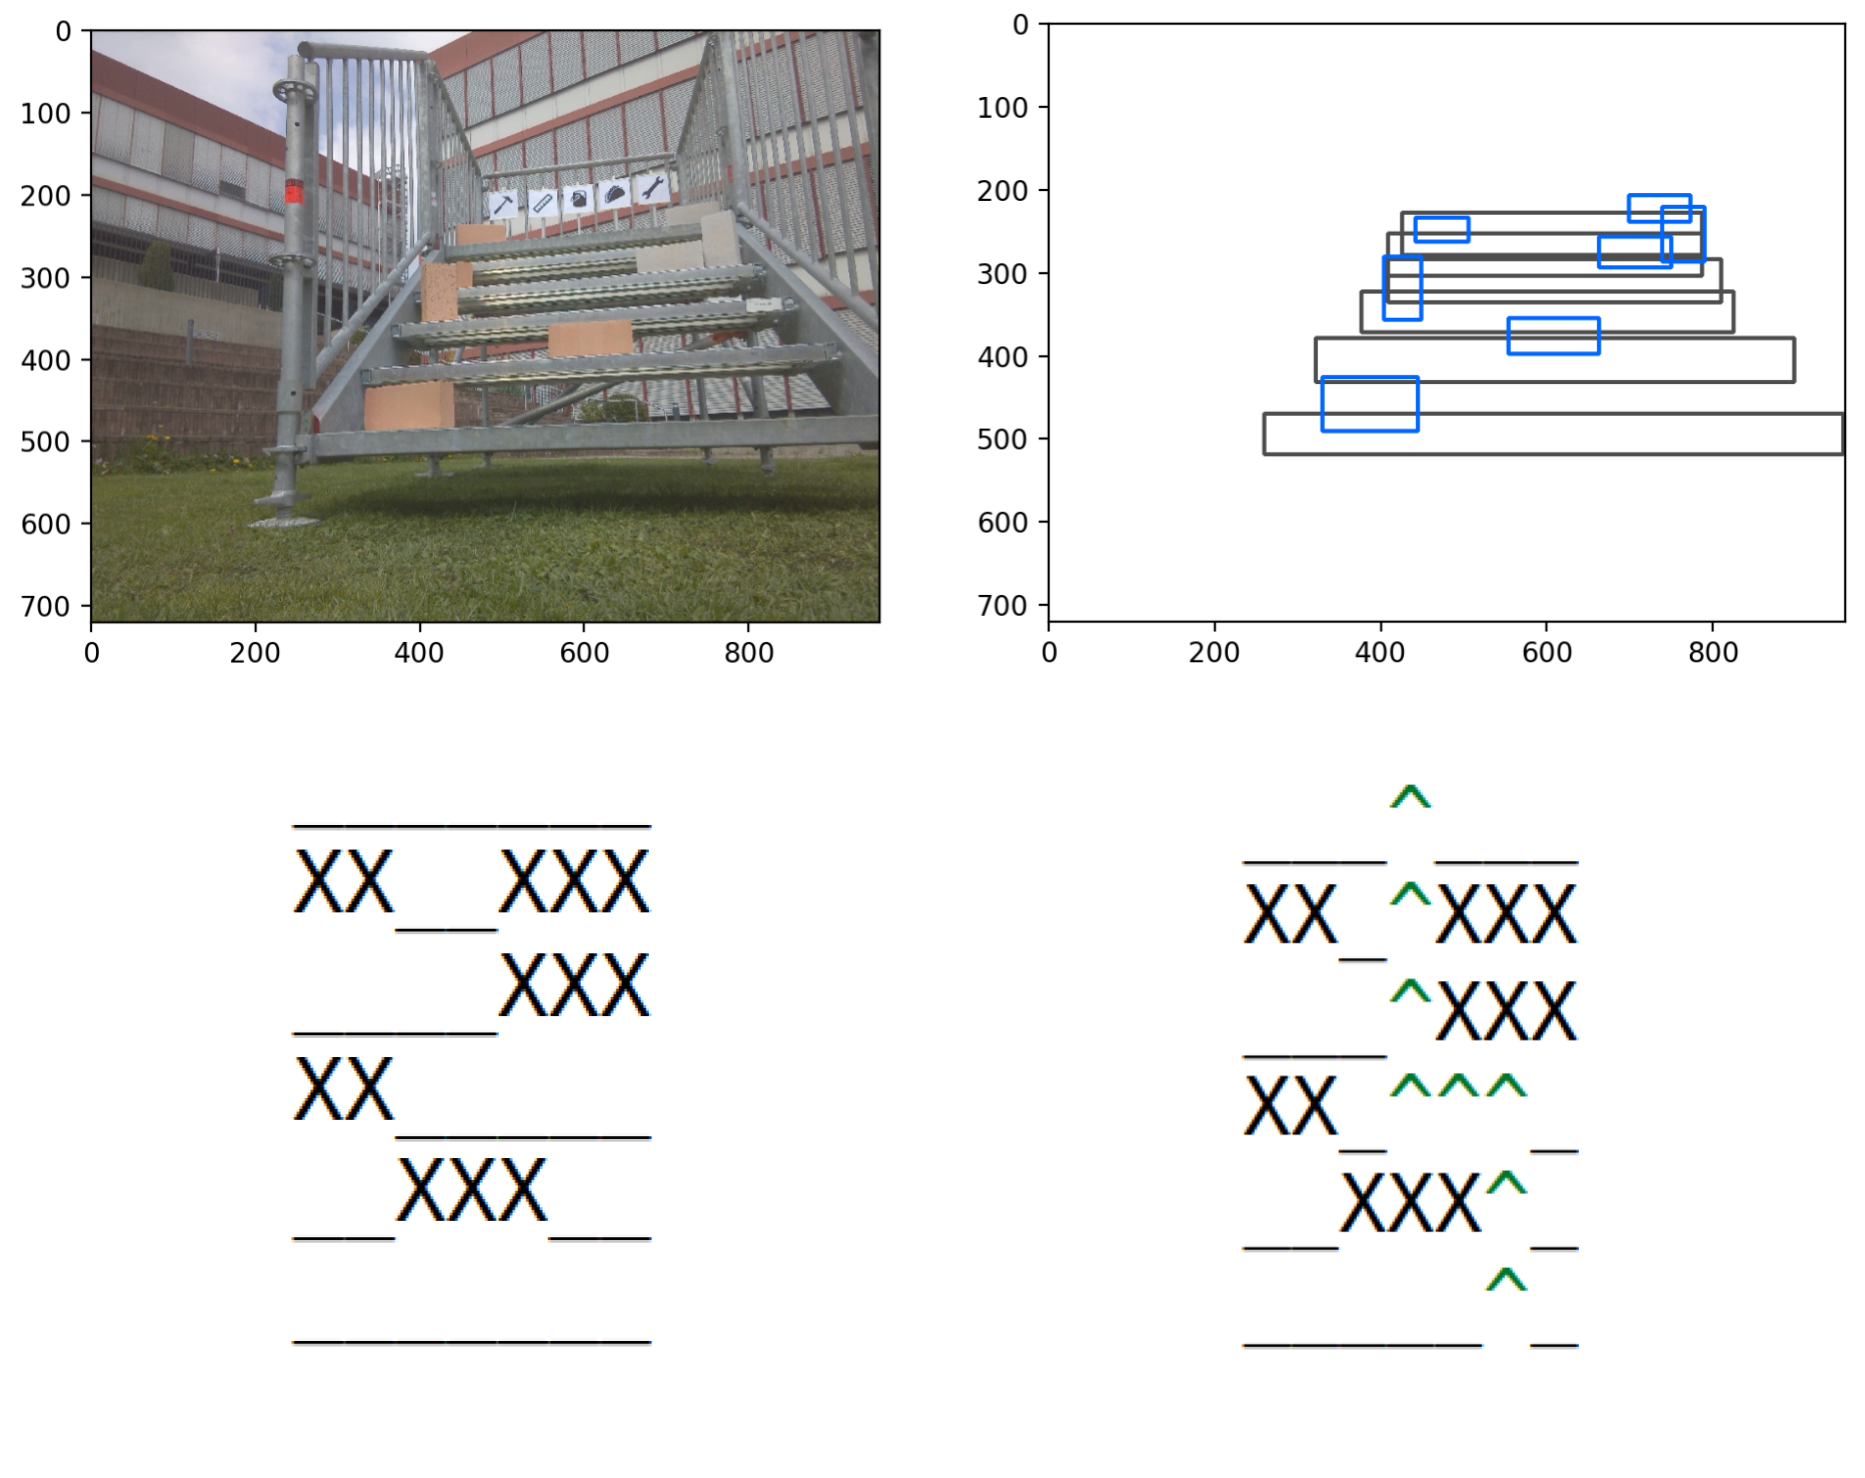
\includegraphics[width=0.95\textwidth]{img/CNN/path-finding}
  \caption{Path finding Algorithmus anhand der Objekterkennung}
  \label{fig:path-finding}
\end{figure}

Wie in Abbildung \ref{path-finding} gezeigt, werden zuerst die Predictions
des Models (oben rechts) in eine Matrixstruktur umgerechnet (unten links).
Der optimale Pfad wird danach mittels A-Star \footnote{\url{https://en.wikipedia.org/wiki/A*_search_algorithm}} Path-Finding
Algorithmus berechnet (unten rechts). Bei der Berechnung wird angenommen (wie inder Aufgabenstellung erwähnt),
dass sich auf der ersten und letzten Treppenstufe keine Ziegelsteine befinden.